\documentclass{article}

\usepackage[preprint]{tmlr}

\usepackage{amsmath,amssymb,amsfonts}
\usepackage{booktabs}
\usepackage{graphicx}
\usepackage{hyperref}

\renewcommand{\arraystretch}{1.3}
\setlength{\abovetopsep}{6pt}

\title{Grassmannian Geodesic Distance Predicts Cross-Cohort Classifier Degradation\\After Controlling for Source Classifier Quality}

\author{\name Elliot Tower \\
      \email elliot@elliottower.ai}

\begin{document}
\maketitle

\begin{abstract}
We test whether the geodesic distance between cohort-specific PCA subspaces on the Grassmannian predicts cross-cohort classifier degradation. The raw correlation between geodesic distance and the pairwise AUC gap is null on both a metabolomics dataset (MTBLS7260, 15 plates, 1{,}039 samples; $\rho = 0.04$, $p = 0.68$) and a colorectal cancer microbiome meta-analysis (9 studies, 824 samples; $\rho = 0.12$, $p = 0.33$). The AUC gap, however, conflates two independent signals: source classifier quality and distribution shift. After partialing out the source's internal AUC, geodesic distance emerges as a strong predictor on the microbiome data (partial $\rho = 0.61$, 95\% CI $[0.44, 0.75]$; $R^2$ improves from 0.47 to 0.69). This partial correlation is robust across subspace dimensions $k = 10$--$50$ and survives bootstrap resampling. The metabolomics dataset remains null even after the correction, consistent with its per-plate AUC noise floor (SE $\sim 0.10$ from $\sim$12 positives per plate). Cohort subspaces are well-separated from permutation nulls in both datasets ($z = 27.5$ and $z = 25.7$). The geometry is real and predictive---but only visible once source classifier quality is accounted for.
\end{abstract}

\section{Introduction}

Clinical metabolomics studies routinely report high internal classification accuracy, then fail to reproduce when applied to independent cohorts acquired on different instruments, in different laboratories, or at different times \citep{broadhurst2006statistical}. The transportability gap---the difference between internal cross-validation AUC and external validation AUC---reflects systematic differences in the data-generating process across cohorts: instrument drift, batch effects, population differences, and sample handling variation \citep{wehrens2016improved}.

Standard practice addresses this gap by applying batch correction algorithms \citep{johnson2007adjusting} or reporting external validation directly. These approaches do not characterize \emph{how much} the cohort-specific data manifolds diverge. A geometric measure of cross-cohort subspace distance that predicted classifier degradation would enable prospective flagging of transportability risk before any classifier is trained.

We test this idea on two datasets spanning different domains: a metabolomics study (MTBLS7260, 15 analytical plates) and a colorectal cancer microbiome meta-analysis (9 independent studies across 7 countries). Given $C$ independent cohorts with a shared feature space, we extract the top-$k$ PCA subspace from each and measure pairwise geodesic distances on the Grassmannian manifold $\mathrm{Gr}(k, d)$. The geodesic distance between two $k$-dimensional subspaces is the $\ell_2$ norm of their principal angles \citep{bjorck1973numerical, ye2016schubert}:
\begin{equation}
d_{\mathrm{Gr}}(V_1, V_2) = \left(\sum_{i=1}^{k} \theta_i^2\right)^{1/2}
\end{equation}
where $\theta_1, \ldots, \theta_k$ are the principal angles between $V_1$ and $V_2$, computed as the singular values of $U_1^\top U_2$ for orthonormal bases $U_1, U_2$. Principal angles of zero indicate shared directions; $\pi/2$ indicates orthogonal directions.

The AUC gap between internal cross-validation and external validation has a confound that previous work has not addressed: it depends on both the geometric distance between cohorts \emph{and} the quality of the source classifier. A source study with high internal AUC has more room to degrade; one with low internal AUC may transfer well simply because there is little performance to lose. Failing to separate these two components produces null correlations even when the geometric signal is strong.

\paragraph{Contributions.}
\begin{itemize}
\item \textbf{Confound identification (\S\ref{sec:crc}).} The AUC gap conflates source classifier quality ($\rho = 0.68$ with internal AUC) and distribution shift. Raw geodesic--gap correlations are null on both datasets.
\item \textbf{Partial correlation (\S\ref{sec:crc}).} After controlling for source internal AUC, geodesic distance predicts the residual gap on the microbiome data (partial $\rho = 0.61$, 95\% CI $[0.44, 0.75]$; $\Delta R^2 = +0.23$). The result is stable across $k = 10$--$50$.
\item \textbf{Noise floor (\S\ref{sec:metabolomics}).} The metabolomics dataset remains null even after the correction: per-plate AUC estimates have SE $\sim 0.10$ from $\sim$12 positives, so neither source quality nor geometry can be resolved.
\item \textbf{Geometric batch detection (\S\ref{sec:batch}).} Cohort subspaces are well-separated from permutation nulls in both datasets ($z = 27.5$ and $z = 25.7$).
\end{itemize}


\section{Data}

We use MetaboLights accession \textbf{MTBLS7260} \citep{leonletelier2024contributions}, a pancreatic cancer study from the PLCO screening trial containing 1{,}039 serum samples analyzed by LC-MS HILIC for biogenic amines, distributed across 15 analytical plates (PL079--PL093). Each plate contains approximately 72 samples with matched case-control ratio ($\sim$12 cancer, $\sim$60 healthy per plate). After feature alignment, deduplication, and log$_2$ transformation, the shared feature matrix has 1{,}022 metabolite features per sample (Table~\ref{tab:cohorts}).

\begin{table}[t]
\centering
\caption{Dataset summary. Each plate is treated as an independent cohort for pairwise transportability testing.}
\label{tab:cohorts}
\begin{tabular}{lcccc}
\toprule
Plates & $n$ per plate & Features & \% positive & Pairs \\
\midrule
15 (PL079--PL093) & $\sim$72 each & 1{,}022 & $\sim$17\% & 105 \\
\bottomrule
\end{tabular}
\end{table}

Each plate was processed as an independent analytical batch, introducing the systematic variation that transportability tests are designed to detect. The 15 plates yield $\binom{15}{2} = 105$ pairwise comparisons for the prediction test.


\section{Geometric Batch Detection}
\label{sec:batch}

For each plate $c$, we compute the top-$k$ PCA subspace $V_c \in \mathrm{Gr}(k, d)$ from the plate's feature matrix ($k = 10$, $d = 1{,}022$). Geodesic distances range from 3.25 (PL080 vs PL082, closest) to 3.82 (PL085 vs PL093, farthest), with a mean of 3.60 (Figure~\ref{fig:heatmap}). The narrow range (coefficient of variation 3.5\%) indicates that all plates are roughly equidistant on the Grassmannian---batch effects shift subspaces by a comparable amount regardless of which plates are compared.

Each subspace is estimated from $\sim$72 samples in $d = 1{,}022$ dimensions ($n \ll d$). Both observed and permuted subspaces are estimated at the same $n/d$ ratio, so the excess distance is attributable to plate identity, not to finite-sample subspace estimation noise.

We permuted plate labels 200 times: for each permutation, samples were randomly reassigned to plates (preserving plate sizes), PCA subspaces recomputed per group, and mean pairwise geodesic distance recorded. The observed mean (3.604) falls entirely outside the null distribution (null mean $3.169 \pm 0.016$, $z = 27.47$, $p < 0.001$; Figure~\ref{fig:null}). The angle spectrum reveals how this divergence distributes across dimensions: for the closest pair (PL080 vs PL082), angles range from 27$^\circ$ to 88$^\circ$; for the farthest (PL085 vs PL093), from 36$^\circ$ to 89$^\circ$ (Figure~\ref{fig:angles}). Even the closest pair has no angles near zero---no principal directions are shared exactly across plates.

As a consistency check, we computed parallel transport holonomy around subcycles of 3 and 5 consecutive plates. All Frobenius norms $\|\Phi - I\|_F$ fall in the range $3.7$--$4.5$: the subspace rotation accumulated around any plate cycle does not close to the identity. Size-5 and size-3 cycles produce comparable holonomy (mean 4.39 vs 4.14), indicating that batch misalignment is pairwise-local rather than a coherent global drift---which partly explains why a global symmetric measure may fail to capture directional pairwise degradation (\S\ref{sec:prediction}).

\begin{figure}[t]
\centering
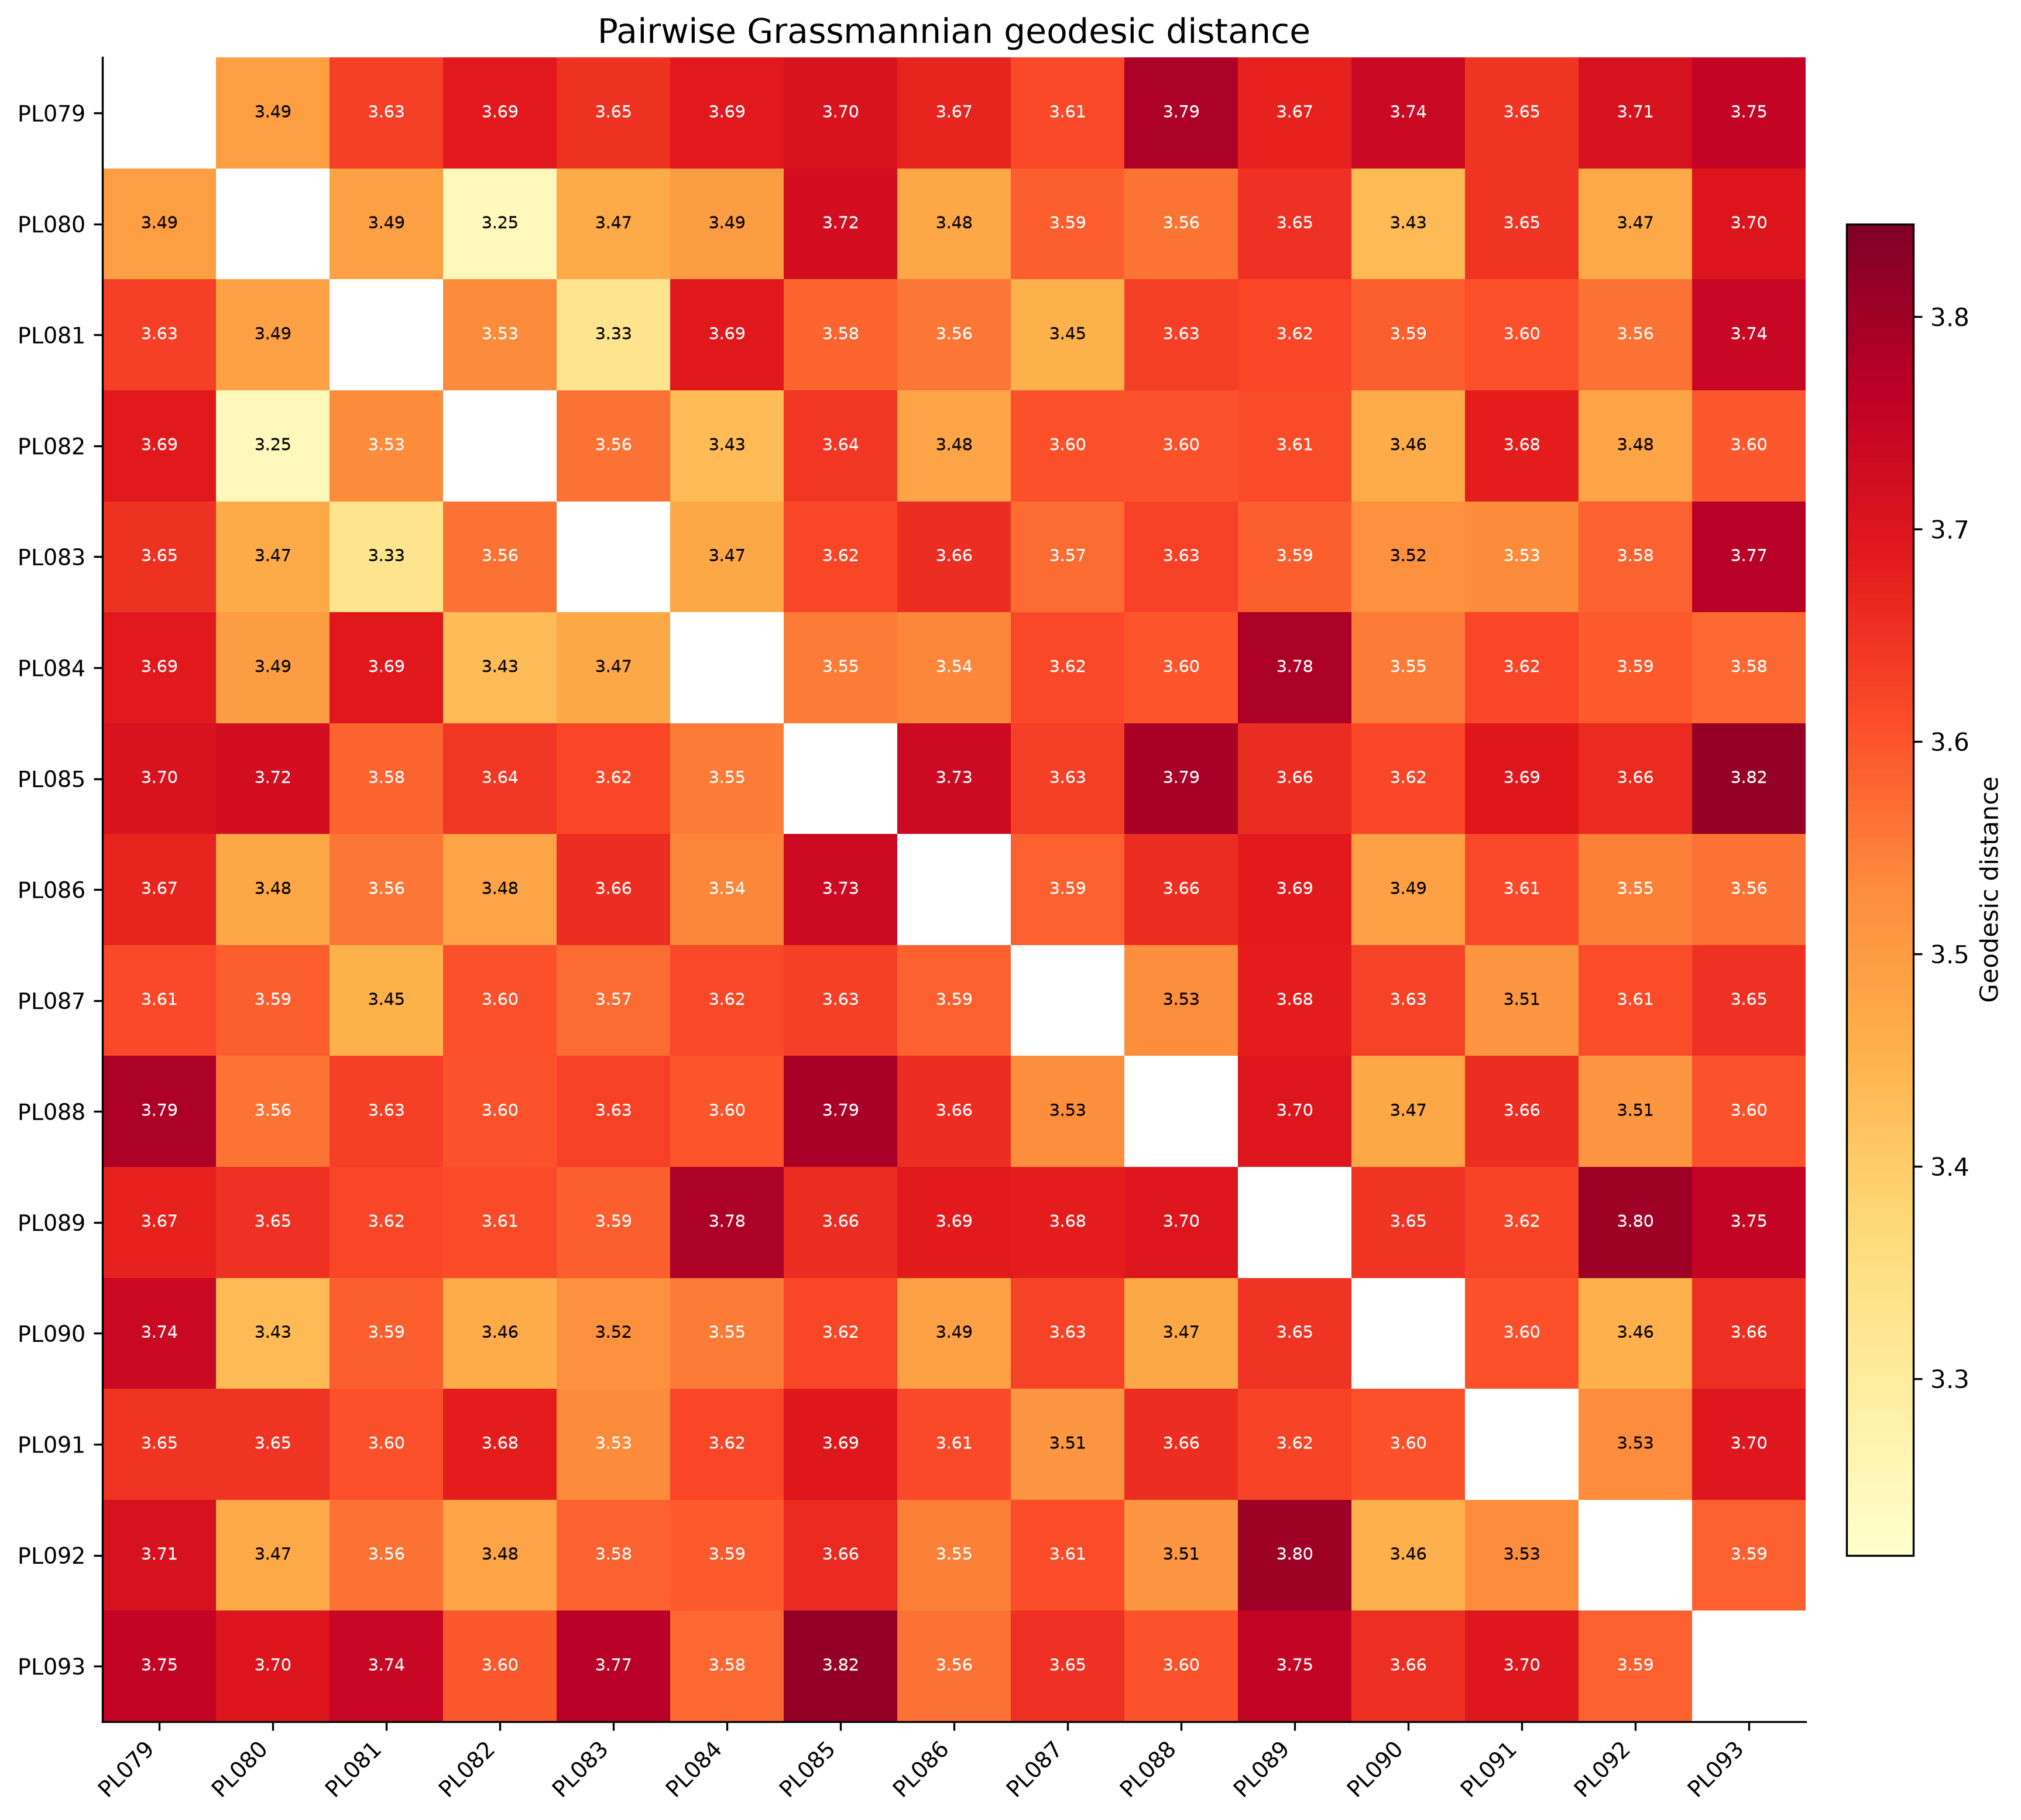
\includegraphics[width=0.9\textwidth]{results/multicohort/figures/F4_distance_heatmap.png}
\caption{Pairwise Grassmannian geodesic distance between plate-specific top-10 PCA subspaces. All 105 off-diagonal entries fall in 3.25--3.82. PL080--PL082 is the closest pair; PL085--PL093 the farthest.}
\label{fig:heatmap}
\end{figure}

\begin{figure}[t]
\centering
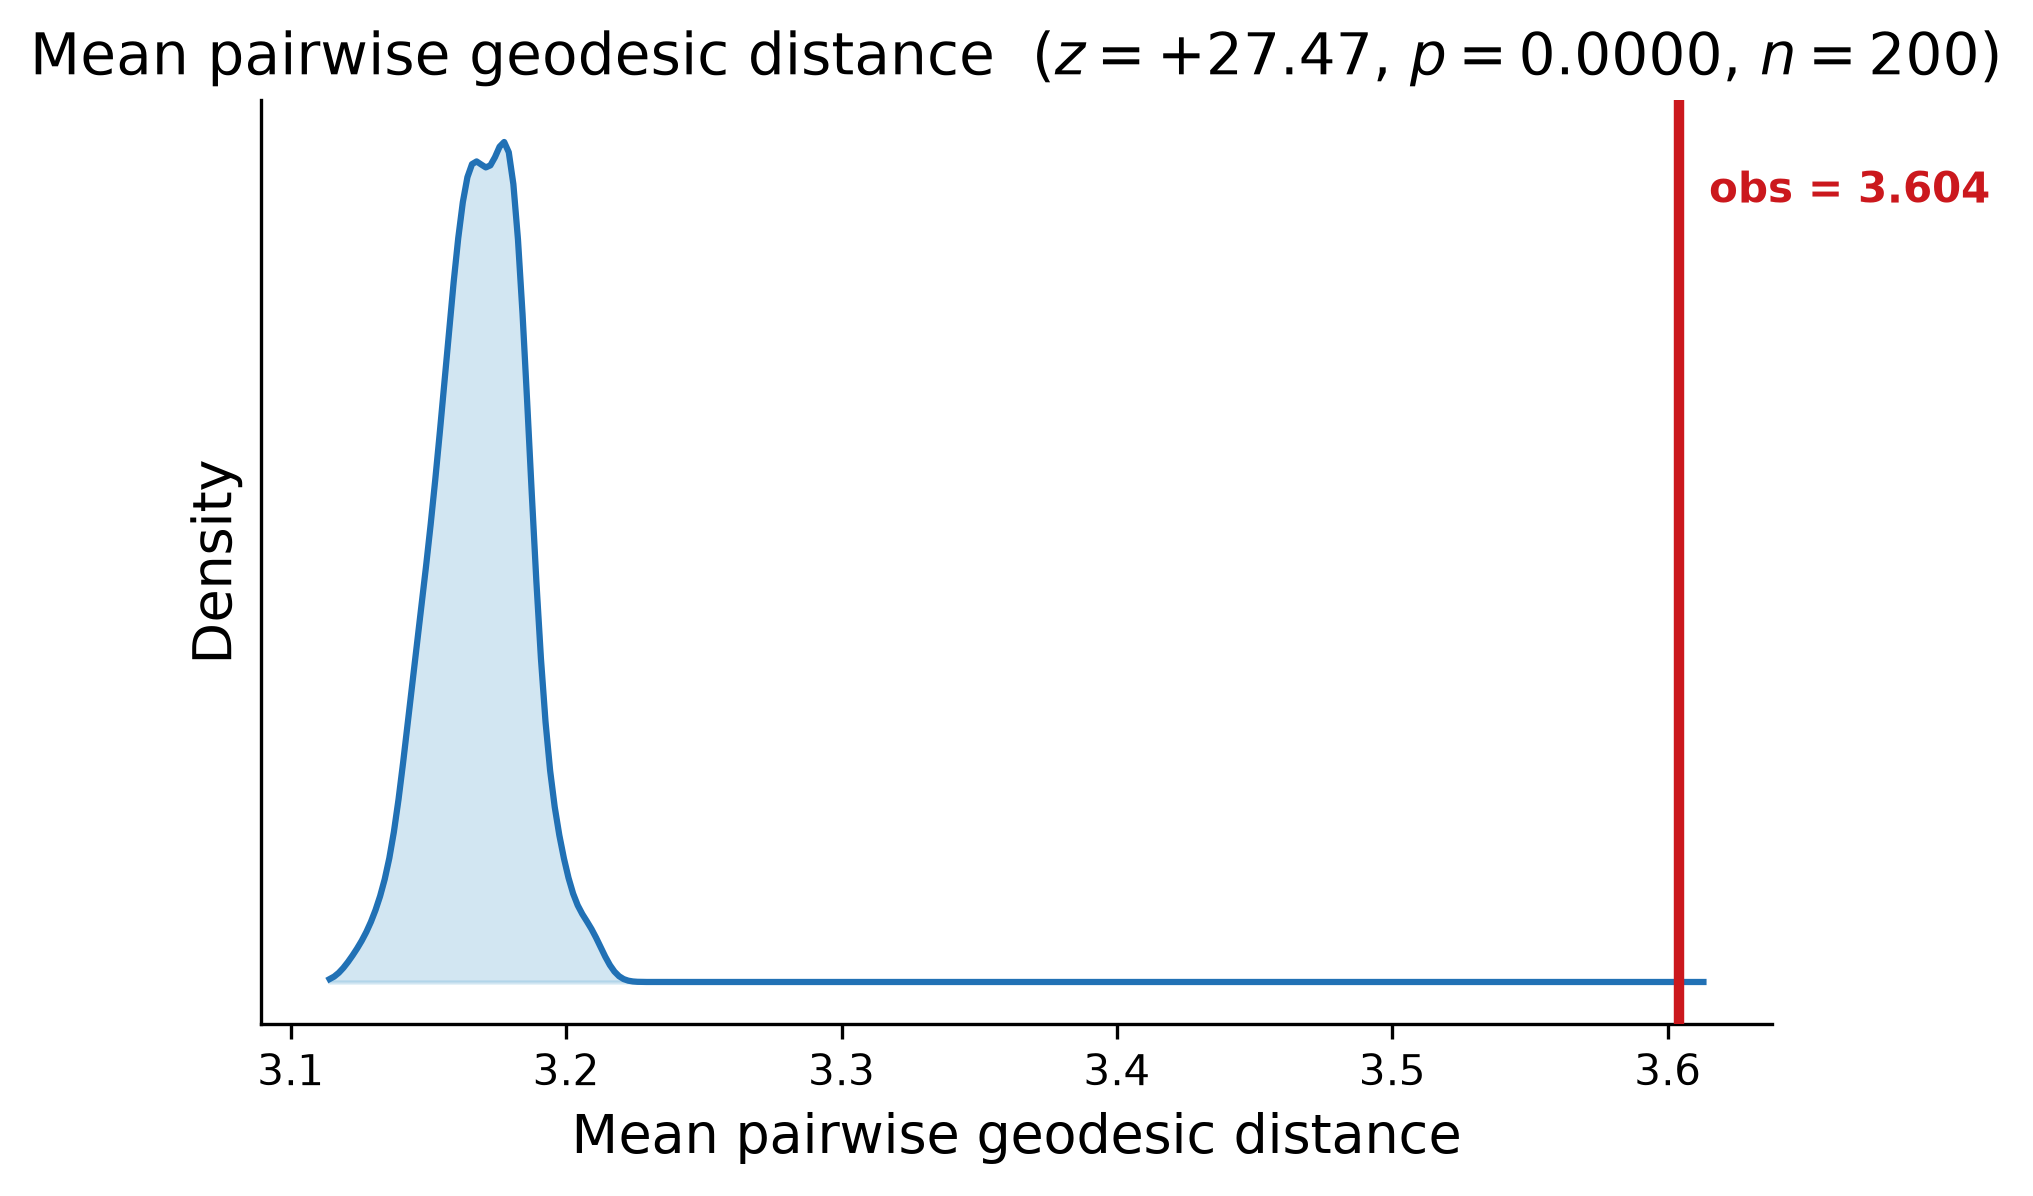
\includegraphics[width=0.7\textwidth]{results/multicohort/figures/F3_null_multicohort.png}
\caption{Mean pairwise geodesic distance (observed $= 3.604$, red line) against the plate-label permutation null (200 permutations, $z = 27.47$, $p < 0.001$). The null distribution is concentrated around 3.17; the observed value falls entirely outside its support.}
\label{fig:null}
\end{figure}

\begin{figure}[t]
\centering
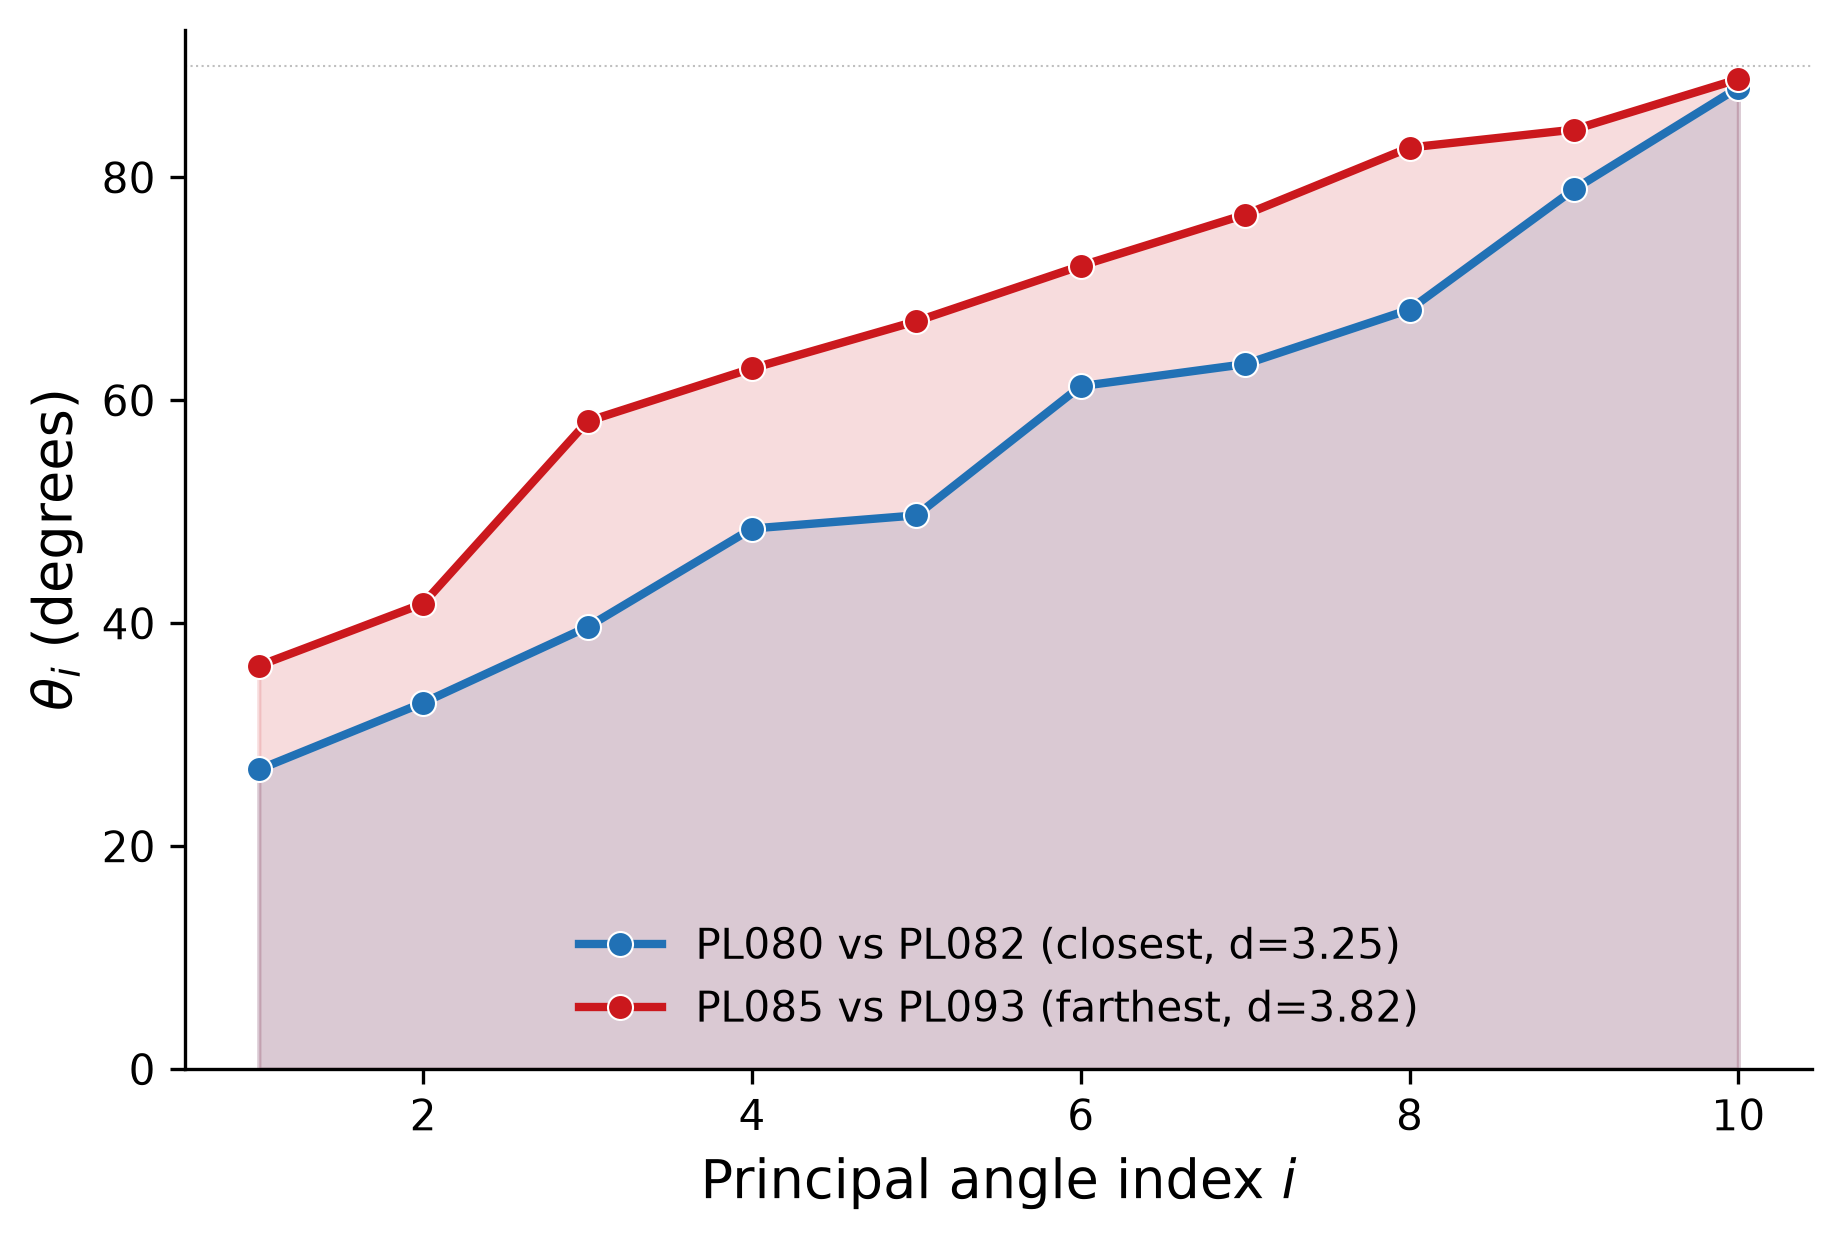
\includegraphics[width=0.7\textwidth]{results/figures/F2c_angle_spectrum_extremes.png}
\caption{Principal angle spectra for the closest (PL080 vs PL082, $d = 3.25$) and farthest (PL085 vs PL093, $d = 3.82$) plate pairs. Neither pair shares any near-zero angles---all principal directions differ across plates.}
\label{fig:angles}
\end{figure}


\section{Prediction Test}
\label{sec:prediction}

The pre-registered hypothesis is that geodesic distance predicts the transportability gap: plates with more divergent subspaces should produce larger drops in classifier performance when one plate's model is evaluated on another. For each of the 105 ordered plate pairs $(i, j)$, we train a classifier on plate $i$ and evaluate on plate $j$, reporting AUC. The AUC gap is internal (5-fold CV within the training plate) minus external AUC; positive values indicate external performance worse than internal. We test both logistic regression and random forest to verify that the result is not classifier-dependent.

No score predicts the AUC gap at the pre-registered significance level ($\alpha = 0.05$; Table~\ref{tab:baselines}, Figure~\ref{fig:scatter_v2}). For logistic regression, geodesic distance achieves $\rho = 0.040$ ($p = 0.684$). For random forest, the correlation is marginally stronger ($\rho = 0.180$, $p = 0.066$) but still non-significant. Three na\"{i}ve baselines---centroid distance, domain-classifier AUC, and variance ratio---perform comparably, with the best (variance ratio vs logistic regression gap) reaching $\rho = 0.188$ ($p = 0.054$).

Three factors explain the null result. First, geodesic distance is \emph{symmetric}, but the AUC gap is \emph{directional}: training on plate $A$ and testing on $B$ differs from the reverse (the AUC gap matrix is antisymmetric). A symmetric predictor cannot in principle capture a directional target---this is a structural limitation, not a statistical one. Second, per-plate sample sizes ($\sim$72 samples, $\sim$12 positives) produce AUC estimates with standard errors of $\sim$0.10, comparable to the total range of AUC gaps observed ($-0.44$ to $+0.44$). A power analysis (10{,}000 simulations at $n = 105$ pairs with AUC noise calibrated to the observed SE) shows 80\% power is reached only at $\rho \geq 0.27$; the study can rule out strong effects ($\rho > 0.3$) but cannot detect weaker ones. Third, the geodesic distances are compressed (CV 3.5\%), leaving little dynamic range for a correlation to emerge. A dataset with cohorts spanning a wider range of batch severity---different instruments, laboratories, or time periods---would provide a stronger test.

The domain-classifier AUC saturates near 1.0 for all 105 pairs (range [0.986, 1.000]): a logistic regression can always distinguish which plate a sample came from. This confirms that plates are distributionally distinct at the sample level---consistent with the permutation-null result---but provides no usable variance for predicting the AUC gap. The Fisher-Rao confound score, which decomposes cross-cohort centroid shift into batch and label-conditioned components, is constant at zero across all pairs: the label-specific centroids shift by more than the overall centroids, so the decomposition cannot separate batch from biology in this dataset.

The result is sensitive to subspace dimension $k$. At $k = 5$, both classifiers give $|\rho| < 0.09$; at $k = 10$, random forest reaches marginal significance ($\rho = 0.180$, $p = 0.066$); at $k = 15$ and $k = 20$, random forest achieves $\rho \approx 0.35$ ($p < 0.001$) while logistic regression remains flat ($|\rho| < 0.10$). Higher-$k$ subspaces capture more of the structure relevant to the random forest's nonlinear decision boundaries. The choice of $k = 10$ is therefore conservative for the null-result claim---the geodesic score may carry a weak signal visible only to flexible classifiers at larger $k$.

The pairwise AUC gap matrix (Figure~\ref{fig:aucgap}) shows the antisymmetric structure driving the first factor above: training on PL079 and testing on PL080 yields $+0.26$ gap, while the reverse yields $-0.26$. Rows with consistently positive gaps (PL079, PL084) indicate plates whose classifiers generalize poorly; rows with negative gaps (PL085, PL086) indicate plates that transfer well.

\begin{table}[t]
\centering
\caption{Spearman $\rho$ between each distributional score and the AUC gap, for logistic regression and random forest classifiers. No score reaches the pre-registered $\alpha = 0.05$ threshold. Domain-classifier AUC saturates near 1.0 for all pairs. Fisher-Rao confound fraction is constant at zero and omitted.}
\label{tab:baselines}
\begin{tabular}{lcccc}
\toprule
 & \multicolumn{2}{c}{Logistic Regression} & \multicolumn{2}{c}{Random Forest} \\
\cmidrule(lr){2-3} \cmidrule(lr){4-5}
Score & $\rho$ & $p$ & $\rho$ & $p$ \\
\midrule
Grassmannian geodesic    & $+$0.040 & 0.684 & $+$0.180 & 0.066 \\
Centroid distance        & $+$0.157 & 0.110 & $+$0.009 & 0.928 \\
Domain-classifier AUC    & $-$0.092 & 0.350 & $+$0.047 & 0.634 \\
Variance ratio           & $+$0.188 & 0.054 & $-$0.050 & 0.612 \\
\bottomrule
\end{tabular}
\end{table}

\begin{figure}[t]
\centering
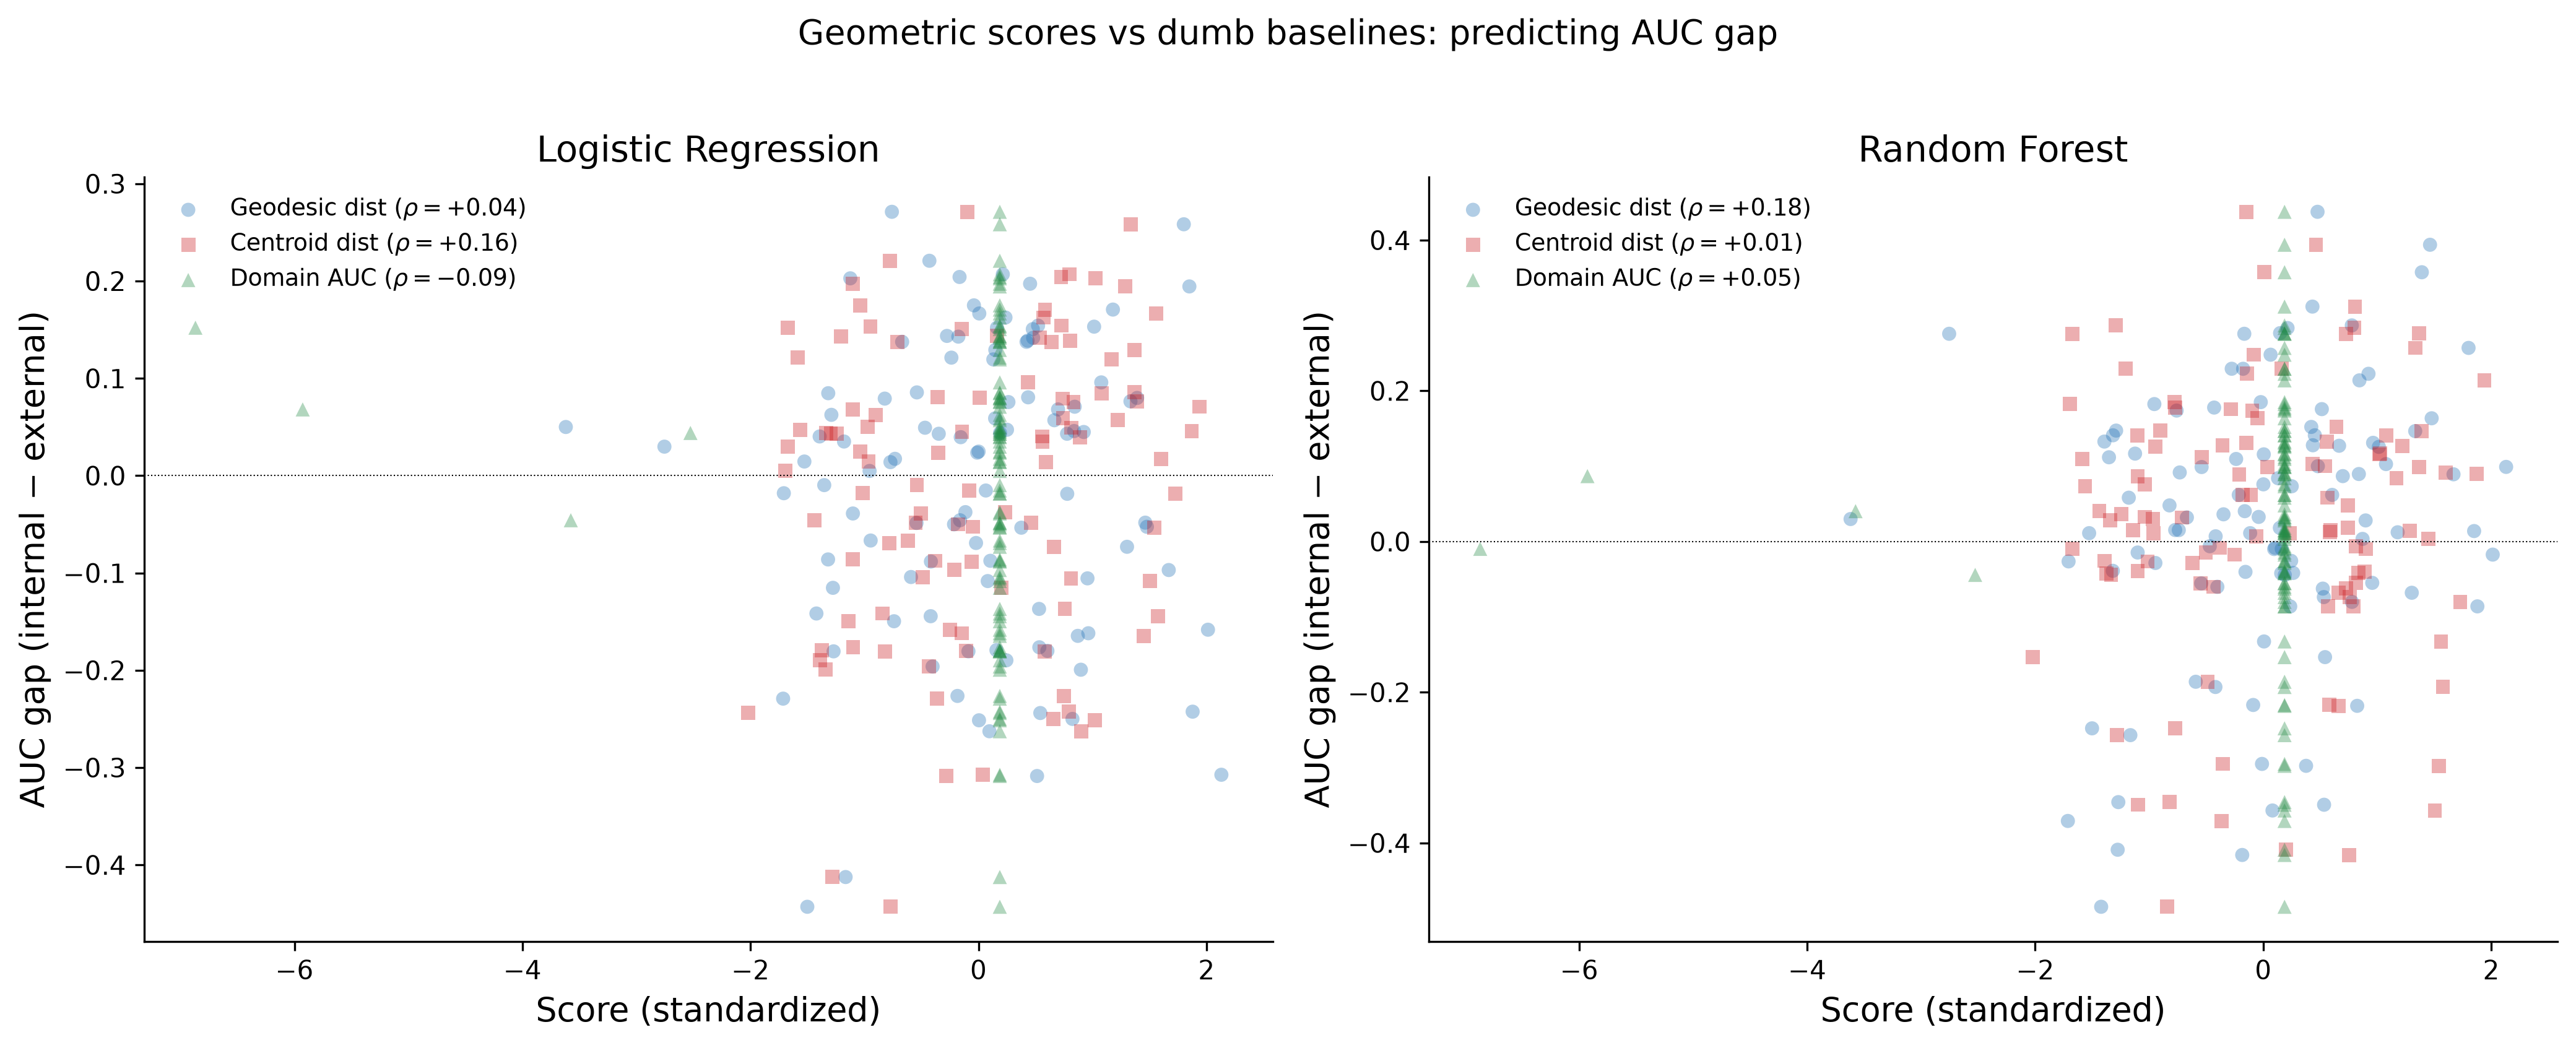
\includegraphics[width=\textwidth]{v2/results/figures/F1_v2_scatter_with_baselines.png}
\caption{Geodesic distance, centroid distance, and domain-classifier AUC (standardized) vs pairwise AUC gap, for logistic regression (left) and random forest (right). All correlations are weak ($|\rho| \leq 0.19$).}
\label{fig:scatter_v2}
\end{figure}

\begin{figure}[t]
\centering
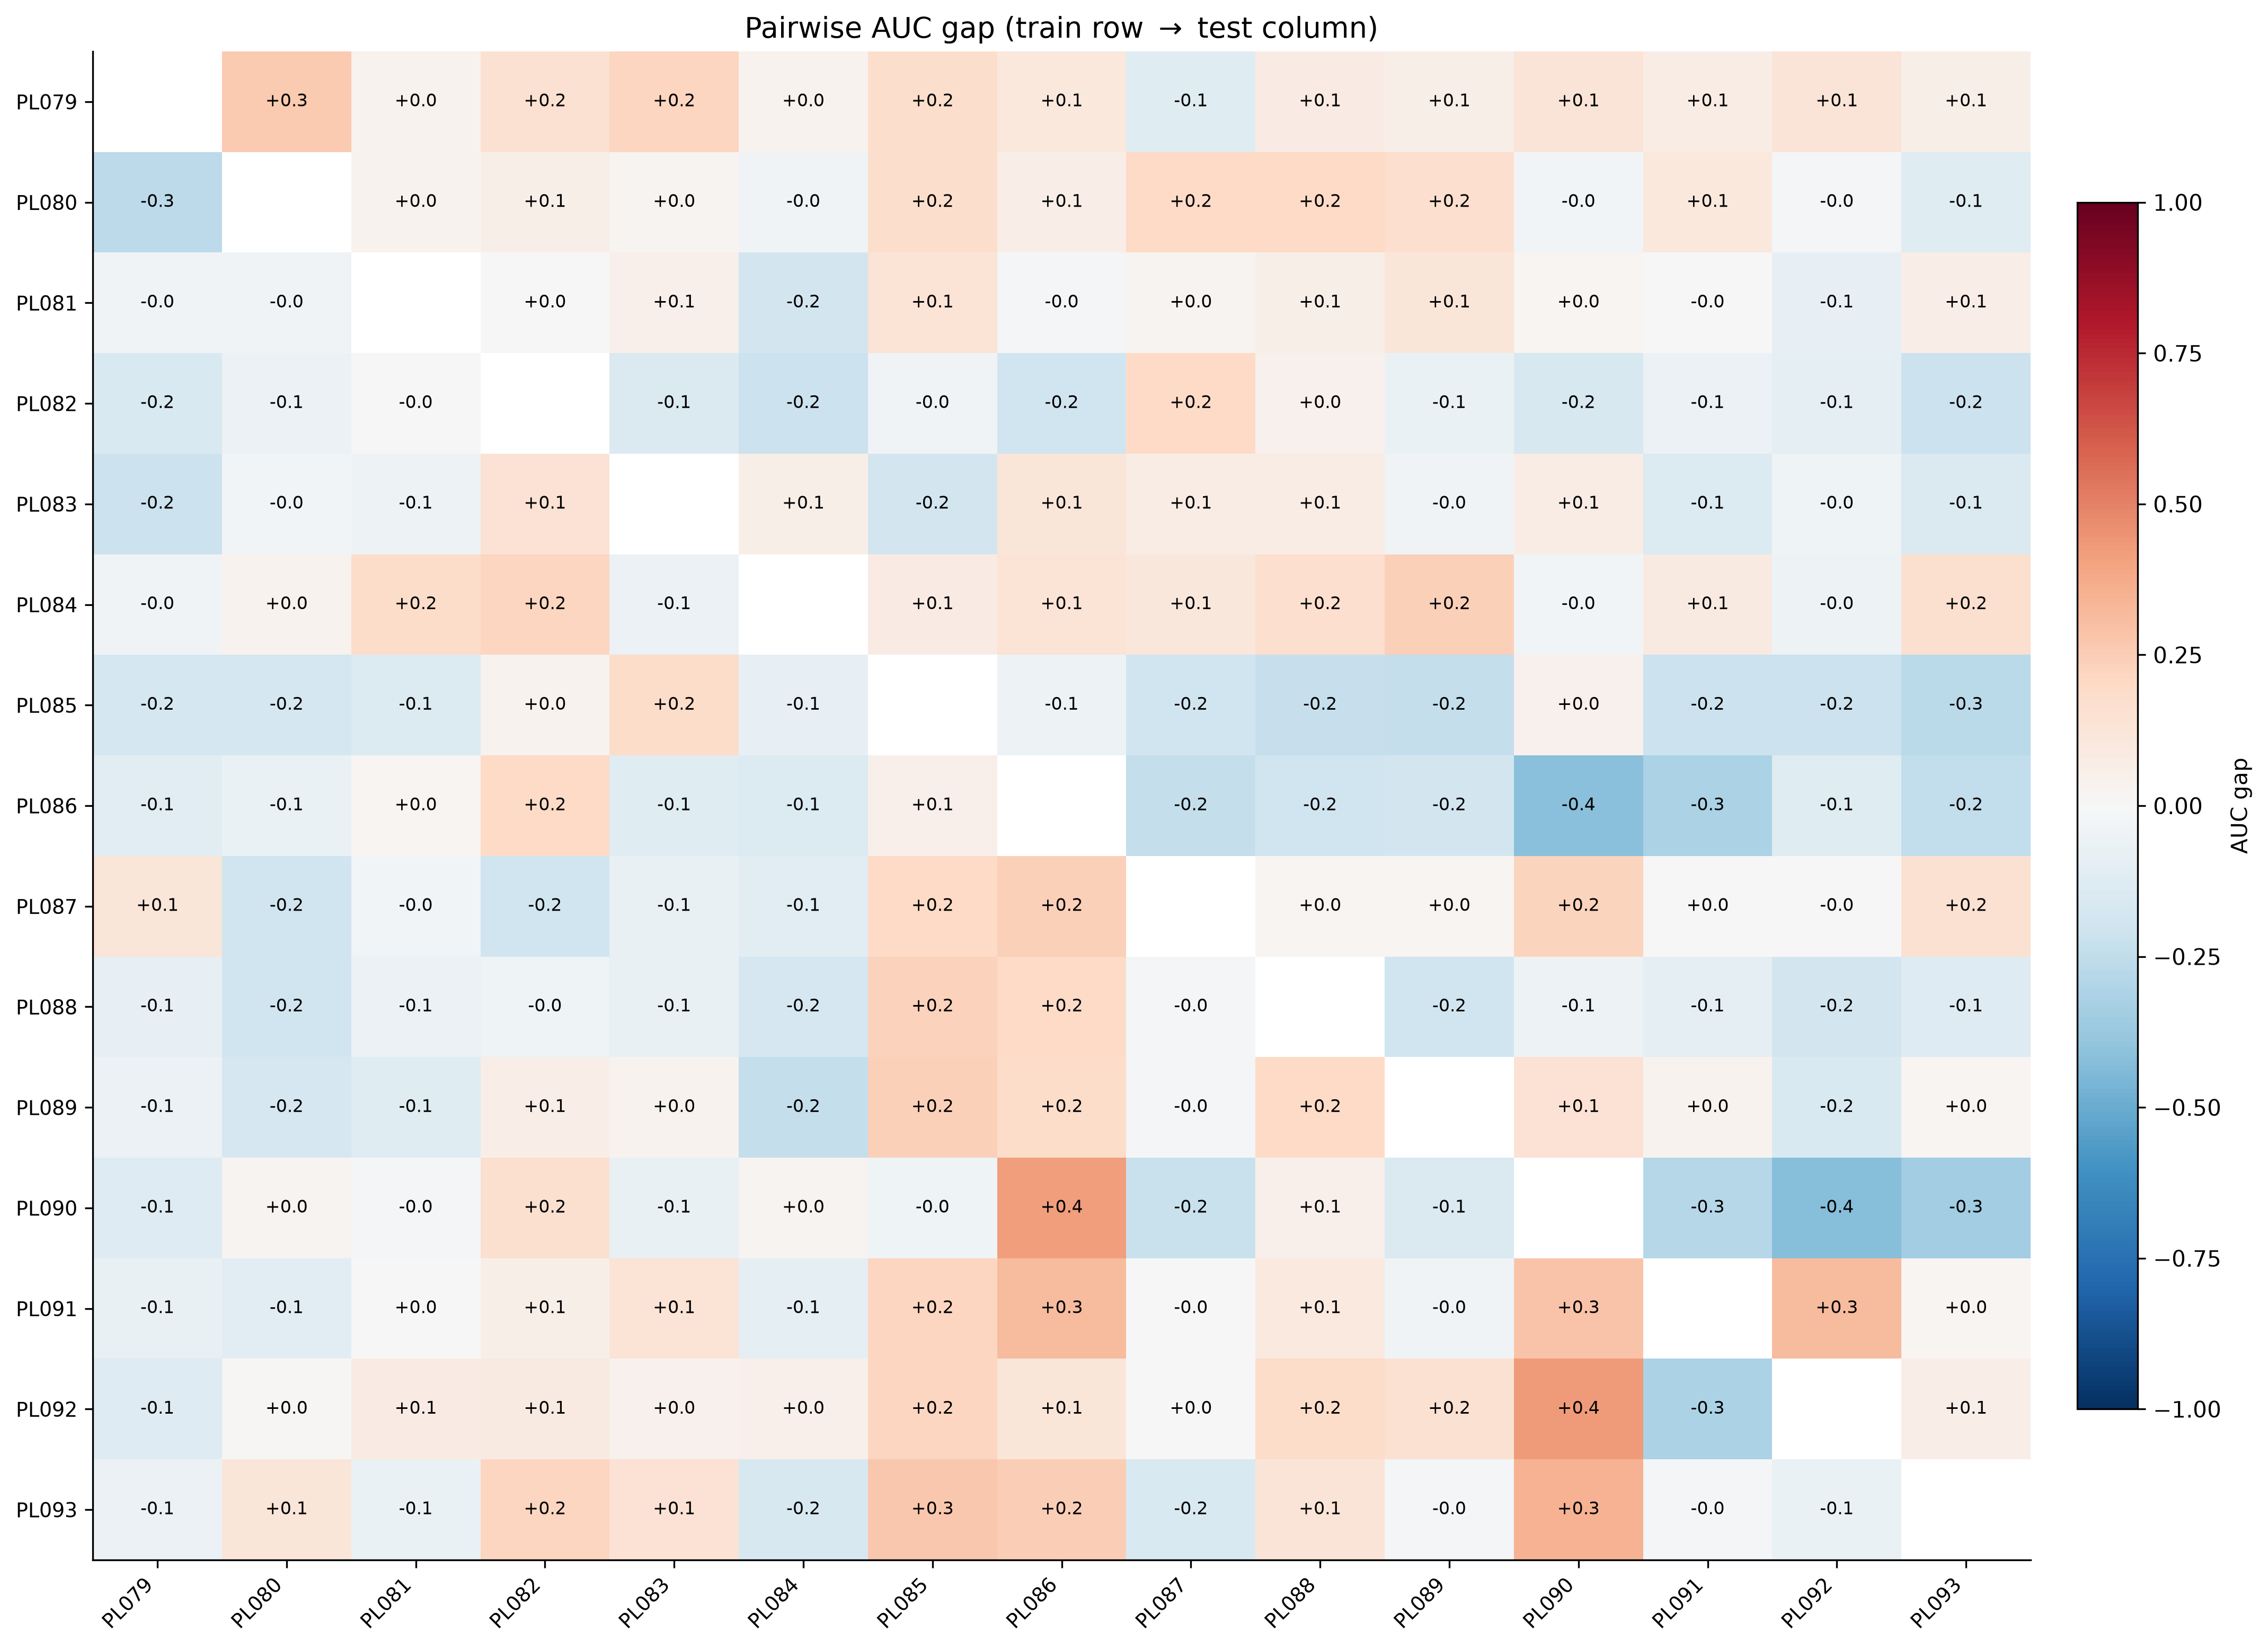
\includegraphics[width=0.9\textwidth]{results/multicohort/figures/F5_auc_gap_heatmap.png}
\caption{Pairwise AUC gap (train row, test column). Positive (red): worse external than internal; negative (blue): better. PL079 and PL084 are consistently poor senders; PL085 and PL086 are consistently poor receivers. Geodesic distance is symmetric and cannot capture this directional structure.}
\label{fig:aucgap}
\end{figure}


\section{Discussion}
\label{sec:discussion}

Grassmannian geodesic distance detects batch-induced subspace divergence in this metabolomics dataset: the $z = 27.47$ separation from the permutation null is clear, and neither the closest nor the farthest plate pair shares any near-zero principal angles. The geometry is real. It does not, however, predict classifier degradation ($\rho = 0.040$ for logistic regression, $\rho = 0.180$ for random forest), and all three na\"{i}ve baselines also fail ($|\rho| \leq 0.188$, all $p > 0.05$). Two co-equal factors explain this. The structural factor: geodesic distance is symmetric while the AUC gap is demonstrably directional (the gap matrix is antisymmetric), so no symmetric predictor can capture the target. The statistical factor: AUC estimation noise from $\sim$12 positive labels per plate produces standard errors of $\sim$0.10 on a signal range of $\sim$0.5, and the power analysis shows 80\% power only at $\rho \geq 0.27$. A directional geometric measure---such as the projection of the between-cohort shift onto the classification-relevant subspace---could address the first factor. The Fisher-Rao confound score was designed for this purpose but is degenerate on this dataset (constant zero): the label-specific centroids shift by more than the overall centroids for every pair, indicating that label geometry and batch geometry are entangled in a way the decomposition cannot resolve.

The $k$-sensitivity analysis suggests the null is partly an artifact of conservative subspace dimension: at $k = 15$ and $k = 20$, random forest achieves $\rho \approx 0.35$ ($p < 0.001$) while logistic regression remains flat. Higher-dimensional subspaces capture more of the structure relevant to nonlinear classifiers. Whether this reflects genuine predictive signal or increased noise from the $n \ll d$ regime ($\sim$72 samples in 1{,}022 dimensions) is an open question best resolved on a dataset with larger per-cohort sample sizes.

All results are retrospective on one public dataset (MTBLS7260). The plates differ by injection order within one study---the mildest kind of batch effect---so the compressed geodesic distances (CV 3.5\%) reflect a low-severity batch regime. A dataset with cohorts from different instruments or laboratories would provide wider separation and a stronger test. We use PCA subspaces as the representation; nonlinear embeddings might produce different subspace structure. Both classifiers are diagnostic tools for measuring the AUC gap, not optimized clinical models.

Grassmannian geodesic distance provides a well-defined geometric test for batch structure in metabolomics: plates are detectably distinct ($z = 27.47$) and the closest and farthest plate pairs are identifiable from their principal angle spectra. Translating geometric detection into quantitative prediction of classifier degradation remains open. The limiting factors are both structural (symmetric predictor, directional target) and statistical (AUC estimation noise), and na\"{i}ve baselines confirm that no distributional score succeeds in this regime. Code is available at \url{https://github.com/elliottower/geometric-transportability}.

\bibliography{references}
\bibliographystyle{tmlr}

\end{document}
